\section{Классификация изображений датасета MNIST}

Теперь решим задачу классификации датасета MNIST. Опишем общий алгоритм \ref{classification-pipeline}, который лежит в основе решения задачи.

\medskip
\begin{algorithm}[H]
	\small
	\SetAlgoLined
	\KwData{Набор изображений рукописных цифр}
	\KwResult{Алгоритм, определяющий рукописную цифру}
	\ForEach{изображения из выборки}{
		Построить фильтрации;
		
		Найти персистентные гомологии, построить диаграмму персистентости;
		
		Получить топологические признаки из диаграммы персистентности;
	}
	
	На наборе полученных признаков обучить модель машинного обучения;
	\caption{Общий алгоритм решения задачи классификации}
	\label{classification-pipeline}
\end{algorithm}
\medskip

Как видно из алгоритма, основным этапом является получение топологических признаков. На их основе и будет обучаться модель машинного обучения. Признаки получаются из диаграммы устойчивости различными методами, поэтому для одного изображения можно получить сразу несколько признаков по одной диаграмме. С другой стороны, персистентные гомологии, а значит и диаграмму устойчивости, можно считать для различных фильтраций одного и того же изображения. Таким образом на основе одного изображения можно сразу получить большое количество признаков, строя по ней различные фильтрации и различными способами векторизуя диаграмму. В данной работе использовался подход, изображенный на рис. \ref{pipeline}

\begin{figure}[!htbp]
	\begin{center}
		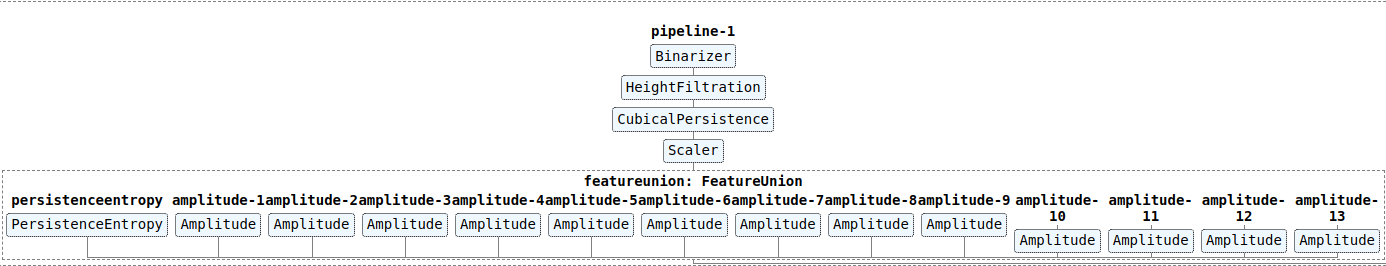
\includegraphics[width=\textwidth]{pipelineDiagram.png}\\
		\caption{Алгоритм получения признаков для Height Filtration}
		\label{pipeline}
	\end{center}
\end{figure}

Опишем подробнее алгоритм получения признаков. Первым шагом является бинаризация изображения с заранее выбранным пороговым значением(в данной работе значение порога равнялось $0.4$). Это нужно для того, чтобы далее воспользоваться специальными методами фильтрации, которые работают именно с бинарным изображением. Бинарным изображением будет называть отображение $B: \mathbb{R}^d \to \{0, 1\}$.

Далее по бинарному изображению $B$ строятся специальные фильтрации. По большому счету фильтрации можно воспринимать как трансформации бинарного изображения обратно в черно-белое, пропущенное через специальный фильтр. Так как в результате получается черно-белое изображение, то можно считать устойчивые гомологии сразу для самой картинки, но обычно построение черно-белого изображения через бинаризацию и фильтрацию наиболее сильно подчеркивает различные топологические особенности. В данном алгоритме использовалась т.н. фильтрация по высоте, радиальная фильтрация, а также фильтрация по плотности(рис. \ref{filtration-comparison}). 

\begin{figure}[!htbp]
	\begin{center}
		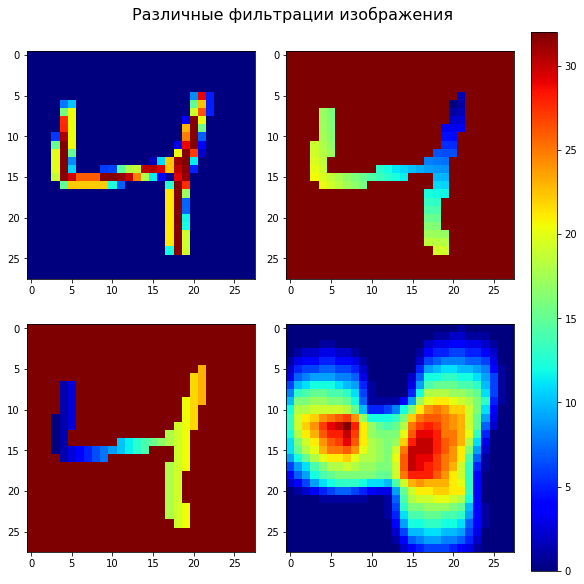
\includegraphics[width=0.75\textwidth]{differentFiltrations.png}\\
		\caption{Черно-белые изображения, полученные с помощью различных фильтраций. Для наглядности, была использована цветная гамма для представления черно-белых значений. В верхнем левом углу -- оригинальное изображение; в верхней правой -- радиальная фильтрация. В нижнем левой углу -- фильтрация по высоте; в нижнем правом углу -- фильтрация по плотности}
		\label{filtration-comparison}
	\end{center}
\end{figure}
Фильтрация по высоте(Height filtration) -- это отображение $H: I \to \mathbb{R}$, где $I$ -- это бинарное изображение в общем случае размерности $d$(в нашем случае размерность равна $2$), которое каждому пикселю изображения $p$ сопоставляет расстояние до гиперплоскости, которая определена вектором $v$ длины $1$, заданным заранее:
\[
H: p \mapsto 
	\left\{
		\begin{array}{ll}
			\langle p,v \rangle, & \text{если } B(p) = 1, \\
			H_\infty, & \text{иначе,}
		\end{array}
	\right.
\]
где $H_\infty$ -- это значение фильтрации $H$ самого дальнего пикселя изображения до гиперплоскости.

Радиальная фильтрация(Radial filtration) -- это отображение $R: I \to \mathbb{R}$, которое каждому пикселю изображения сопоставляет расстояние до выбранного заранее центра $c$:
\[
	R: p \mapsto 
		\left\{
			\begin{array}{ll}
				\norm{c - p}_2, & \text{если } B(p) = 1, \\
				R_\infty, & \text{иначе,}
			\end{array}
		\right.
\]
где $R_\infty$ -- это расстояние самого дальнего пикселя до центра. То есть фильтрация строится исходя из значения некоторой радиальной функции от пикселя $p$, у которого $B(p)=1$.

Фильтрация по плотности(Density filtration) -- это отображение $D: I \to \mathbb{R}$, которое каждому пикселю изображения сопоставляет число пикселей $p$, таких, что $B(p)=1$, находящихся на растоянии не больше задаваемого $r$:
\[
	D_r(p) \coloneqq \abs{\{ v \in I | B(v) = 1 \land \norm{p-v} \leq r \}},
\]
где $\norm\cdot$ -- любая норма в $\mathbb{R}^2$. В данном алгоритме использовалась стандартная евклидова метрика.

Так как вектор направления для фильтрации по высоте и центр для радиальной фильтрации задается заранее, то можно формировать различные фильтрации при различных значениях вектора направления и центра. В данном алгоритме фильтрация по высоте строилась с $8$ различными значениями для вектора направления, радиальная фильтрация строилась с $9$ различными значениями для центра, а фильтрация по плотности строилась с $3$ различными значениями для радиуса. Таким образом, для одного изображения получалось $20$ фильтрации.

\begin{figure}[!htbp]
	\begin{center}
		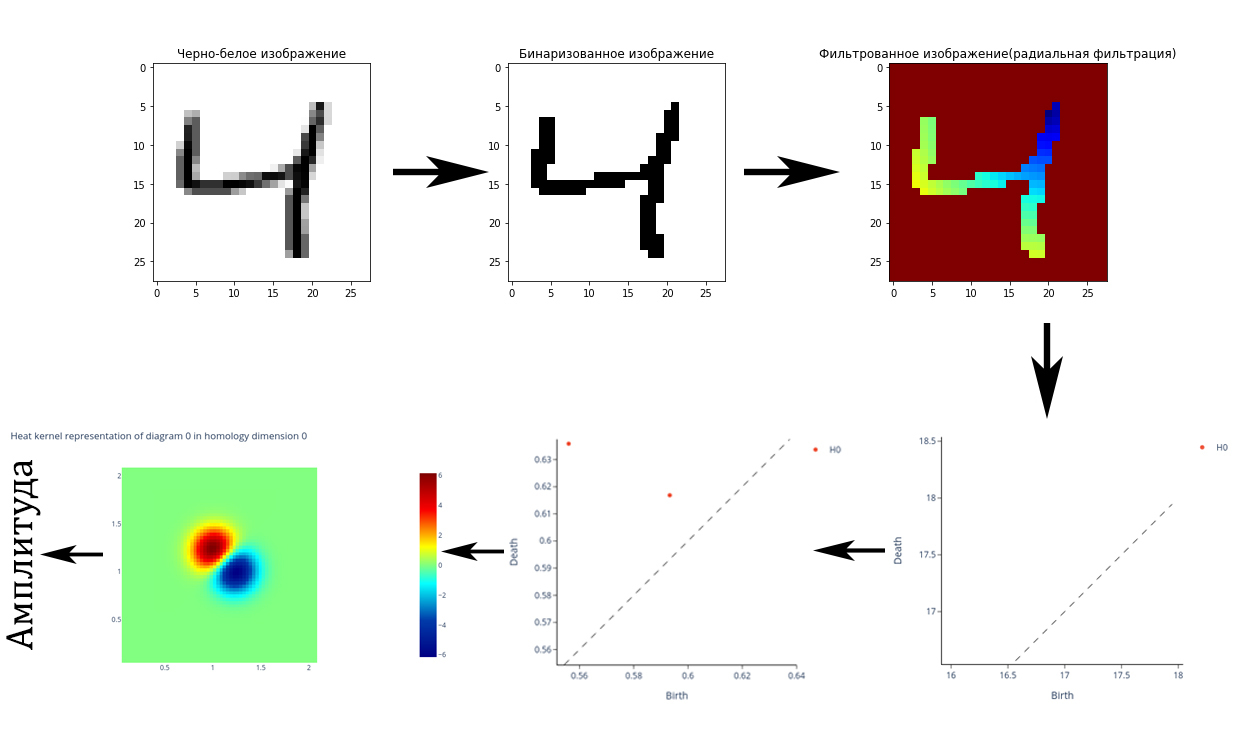
\includegraphics[width=0.75\textwidth]{pipe.jpg}\\
		\caption{Пример работы алгоритма}
		\label{example}
	\end{center}
\end{figure}

Далее для каждой из полученных фильтраций вычислялись устойчивые гомологии $0$ и $1$ размерности, а по ним строились диаграммы персистентности, которые далее были приведены к одному и тому же масштабу. 

\begin{figure}[!htbp]
	\begin{subfigure}{.33\textwidth}
		\centering
		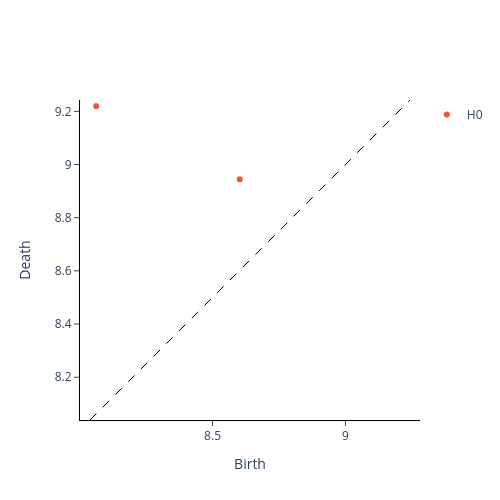
\includegraphics[width=\linewidth]{radial_persistence.png}\\
		\caption{Radial Filtration}
	\end{subfigure}%
	\begin{subfigure}{.33\textwidth}
		\centering
		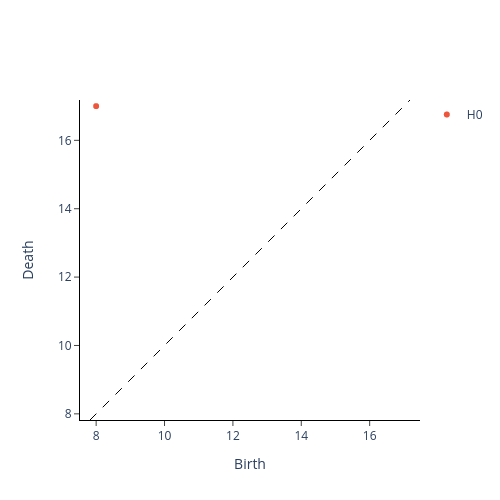
\includegraphics[width=\linewidth]{height_persistence.png}\\
		\caption{Height Filtration}
	\end{subfigure}%
	\begin{subfigure}{.33\textwidth}
		\centering
		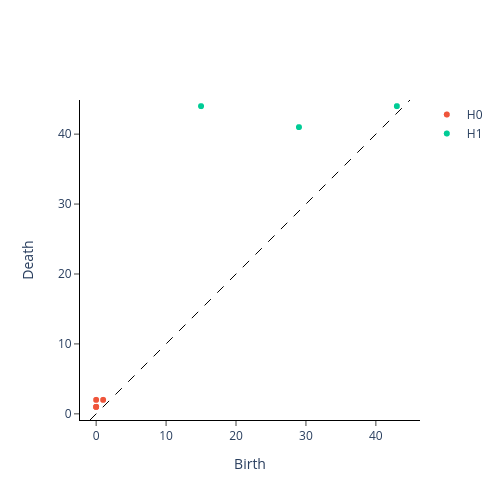
\includegraphics[width=\linewidth]{density_persistence.png}\\
		\caption{Density Filtration}
	\end{subfigure}%
	\caption{Диаграммы устойчивости для различных фильтраций}
	\label{persistences}
\end{figure}

 На рис. \ref{example} представлен пример работы алгоритма для одного бинарного изображения из датасета. На рис. \ref{persistences} представлены диаграммы устойчивости для различных фильтраций. На рис. \ref{scaled_persistences} представлены диаграммы устойчивости, приведенные к одному и тому же масштабу. Видно, что изменились значения шкал рождения/смерти у диаграмм.


\begin{figure}[!htbp]
	\begin{subfigure}{.33\textwidth}
		\centering
		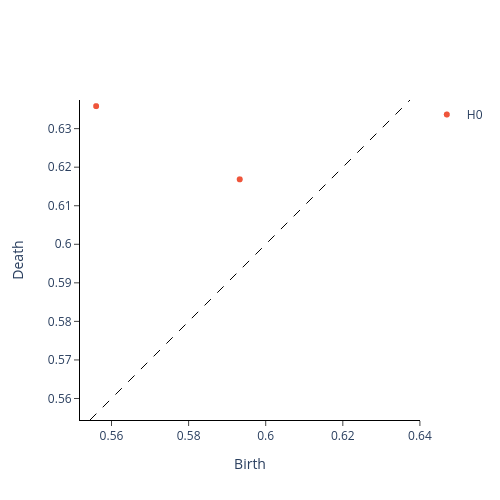
\includegraphics[width=\linewidth]{scaled_radial_persistence.png}\\
		\caption{Radial Filtration}
	\end{subfigure}%
	\begin{subfigure}{.33\textwidth}
		\centering
		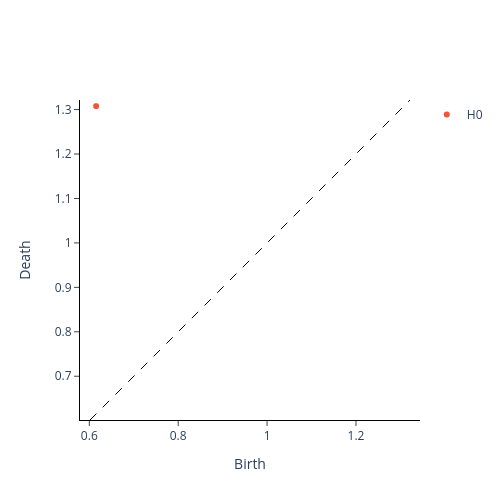
\includegraphics[width=\linewidth]{scaled_height_persistence.png}\\
		\caption{Height Filtration}
	\end{subfigure}%
	\begin{subfigure}{.33\textwidth}
		\centering
		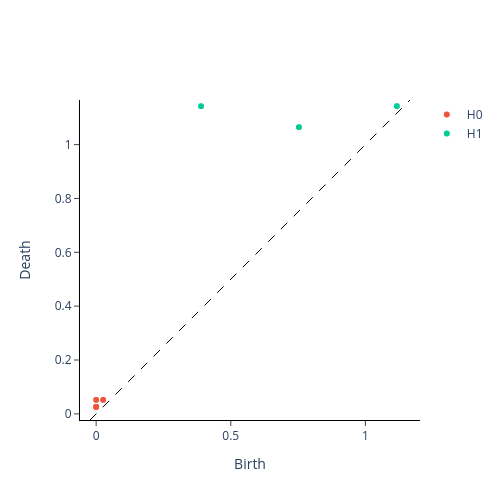
\includegraphics[width=\linewidth]{scaled_density_persistence.png}\\
		\caption{Density Filtration}
	\end{subfigure}%
	\caption{Диаграммы устойчивости для различных фильтраций, приведенные к одному масштабу}
	\label{scaled_persistences}
\end{figure}

В свою же очередь, для каждой диаграммы вычислялись $14$ признаков: персистентная энтропия и $13$ амплитуд для различных векторных представлений. На рис. \ref{representations} представлен пример таких представлений для различных фильтраций. Таким образом, для одной картинки получалось $20 \times 2 \times 14 = 560$ признаков. Однако вероятно, что некоторые из таких признаков будут коррелировать, а поэтому необходимо будет произвести отбор признаков.

\begin{figure}[!htbp]
	\begin{subfigure}{.33\textwidth}
		\centering
		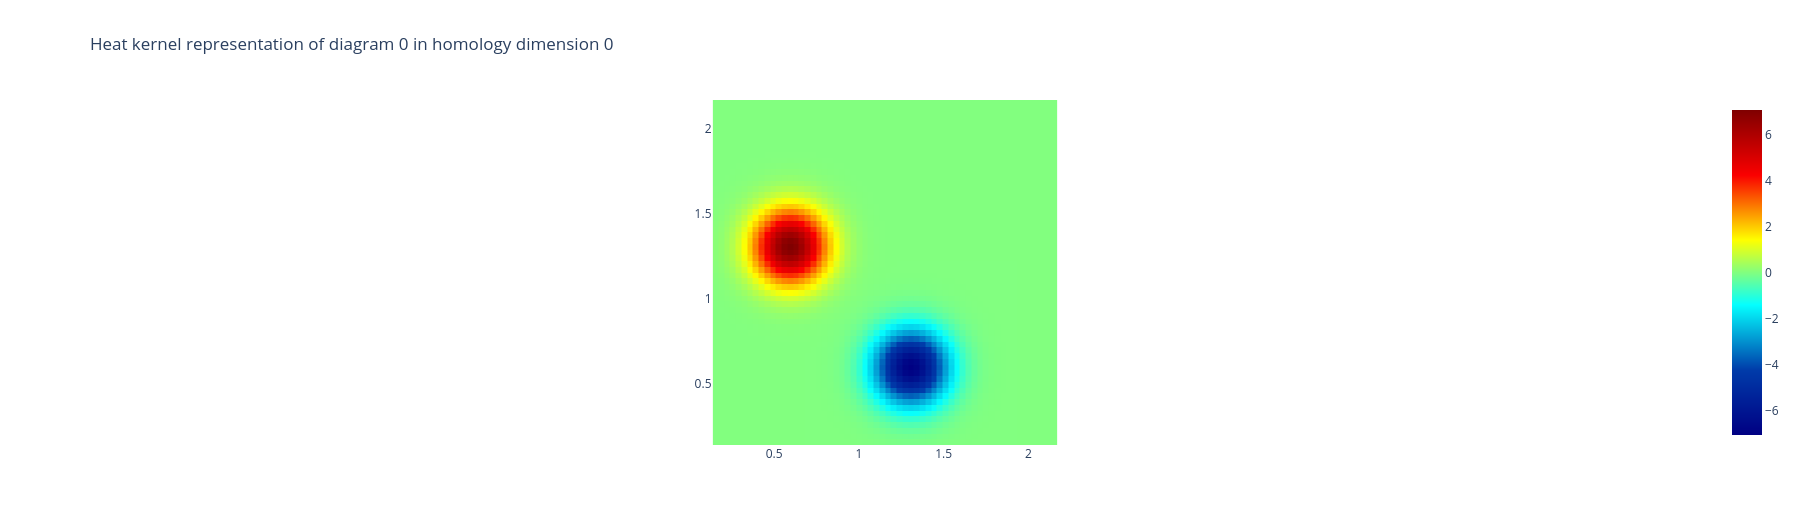
\includegraphics[width=\linewidth]{heat_height.png}\\
		\caption{Height filtration}
	\end{subfigure}%
	\begin{subfigure}{.33\textwidth}
		\centering
		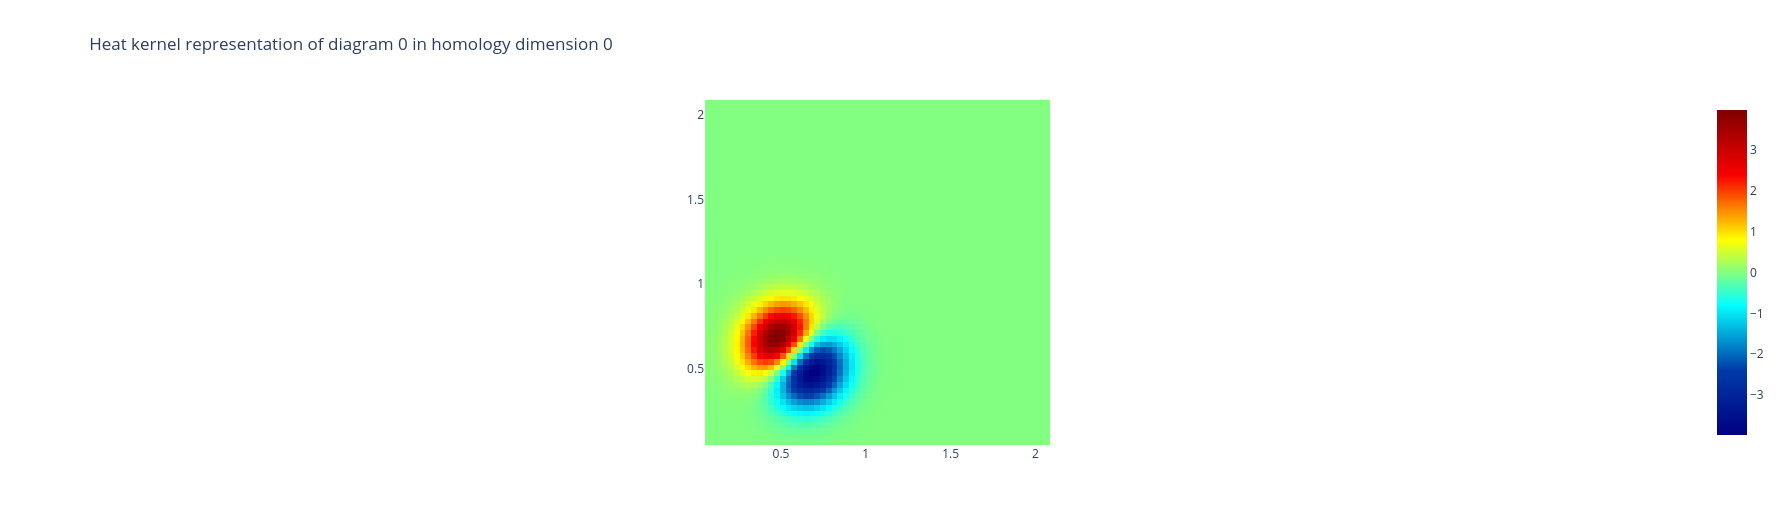
\includegraphics[width=\linewidth]{heat_rad.png}\\
		\caption{Radial filtration}
	\end{subfigure}%
	\begin{subfigure}{.33\textwidth}
		\centering
		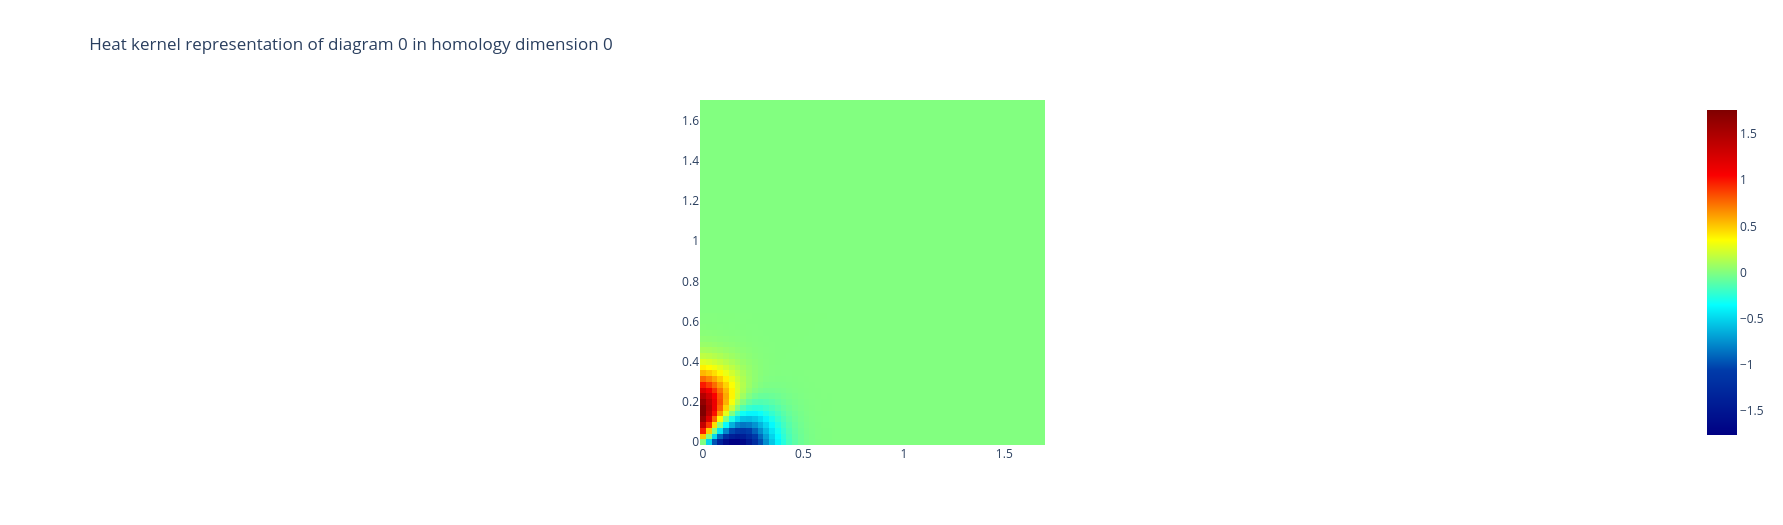
\includegraphics[width=\linewidth]{heat_dense.png}\\
		\caption{Density filtration}
	\end{subfigure}%
	\caption{Heat Kernel для различных фильтраций для одного и того же изображения}
	\label{representations}
\end{figure}

После получения векторного представления для изображений из выборки, дальнейшим этапом является обучение модели машинного обучения. В данной работе использовались следующие модели:
\begin{itemize}
	\item Метод опорных векторов
	\item Случайный лес
	\item Логистическая регрессия
	\item LightGBM
	\item CatBoost
	\item XGBoost
\end{itemize}
Первым шагом было запустить эти модели без настраивания параметров и отбора признаков, и посмотреть, как хорошо они справляются с задачей, т.е. таким образом получить начальное значение для каждой из модели, чтобы в дальнейшем значения качества моделей увеличивать как за счет настраивания параметров модели, так и за счет отбора признаков. Получившиеся результаты отображены в табл. \ref{tabl:baselines}

\begin{table}[!htbp]
	\centering
	\small
	\begin{tabularx}{\linewidth}{|X|X|X|}
		\hline
		Название модели & Значение на тренировочной выборке & Значение на тестовой выборке\\ \hline
		Логистическая регрессия & 0.989 & 0.903 \\
		\hline 
		Метод опорных векторов & 1.0 & 0.893 \\
		\hline
		Случайный лес & 1.0 & 0.89 \\
		\hline
		LightGBM & 1.0 & 0.9 \\
		\hline
		XGBoost & 1.0 & 0.883 \\
		\hline
		CatBoost & 1.0 & 0.893 \\ 
		\hline
	\end{tabularx}
	\caption{Значения базовых моделей на тренировочной и тестовой выборках}	
	\label{tabl:baselines}
\end{table}

Несмотря на очевидное переобучение -- значения на тренировочной выборке куда лучше, чем на тестовой -- все модели проявили себя очень хорошо и показали неплохие результаты(тут стоит отметить, что современные сверточные нейронные сети достигают $99.95\%$ точности). Попробуем для каждой модели сделать поиск по сетке, чтобы улучшить результаты моделей. Результат поиска по сетке представлен в табл. \ref{tabl:gridsearch}. Можно заметить, что для некоторых моделей проблема переобучения исчезла в результате подбора параметров.

\begin{table}[!htbp]
	\centering
	\small
	\begin{tabularx}{\linewidth}{|X|X|X|}
		\hline
		Название модели & Значение на тренировочной выборке & Значение на тестовой выборке\\ \hline
		Логистическая регрессия & 0.911 & 0.917 \\
		\hline 
		Метод опорных векторов & 0.903 & 0.893 \\
		\hline
		Случайный лес & 0.88 & 0.87 \\
		\hline
		LightGBM & 1.0 & 0.9 \\ %CHANGE
		\hline
		XGBoost & 1.0 & 0.883 \\ %CHANGE
		\hline
		CatBoost & 1.0 & 0.893 \\ 
		\hline
	\end{tabularx}
	\caption{Значения наилучших моделей, полученных в результате подбора параметров поиском по сетке, на тренировочной и тестовой выборках}	
	\label{tabl:gridsearch}
\end{table}

Как было сказано ранее, скорее всего многие признаки коррелируют между собой. Поэтому дальнейший шаг -- это отбор признаков. Сперва убедимся, что уменьшение признаков может привести к росту качества модели. Для этого запустим случайный лес на выборке. Случайный лес может быть использован в качестве отбора признаков -- есть возможность подсчитать важность признаков для этой модели. Те признаки, которые оказались наиболее важны для случайного леса, вероятно будут и наиболее важными и для других моделей. Поэтому с помощью случайного леса упорядочим все признаки по убыванию их важности. Далее в цикле будем запускать модели на выборке, но с разным числом признаков -- так как они упорядочены, то будем брать первые $50n$ признаков, где $1 \leq n \leq 11$. Запускать модели будем с поиском по сетке, чтобы использовать наилучшие параметры для данной выборке. График зависимости качества построенных моделей от числа признаков представлен на рис. \ref{accuracy-numFeatures}.

\begin{figure}[!htbp]
	\begin{center}
		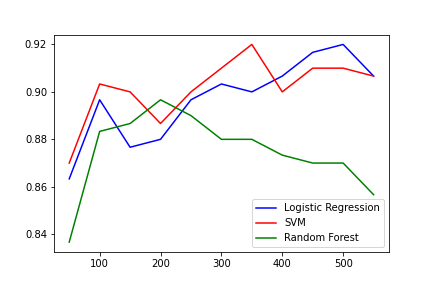
\includegraphics[width=0.75\textwidth]{models-topfeatures.png}\\
		\caption{График зависимости качества построенных моделей от числа признаков}
		\label{accuracy-numFeatures}
	\end{center}
\end{figure}

На графике видно, что, уменьшив количество признаков, все модели улучшают свои показатели качества. 

Далее можно сравнить качество моделей, которые используют топологические признаки, с качеством моделей, которые в качестве признаков будут получать просто векторное представление изображения. То есть для таких моделей признаками будут сами значения пикселей изображения. Так как модели с топологическими признаками показали наилучший результат именно при уменьшении количества признаков, то также отсортируем признаки для новых моделей по убыванию важности для случайного леса, и будем брать первые $50n$ признаков, каждый раз обучая модель с поиском по сетке, чтобы подобрать наилучшие параметры. Так как теперь признаков будет $28 \times 28 = 784$, то $1 \leq n \leq 15$. На графике \ref{accuracies_diff_features} представлены сравнения различных моделей, но с разными признаками. 

\begin{figure}[!htbp]
	    \centering % <-- added
	\begin{subfigure}{0.25\textwidth}
		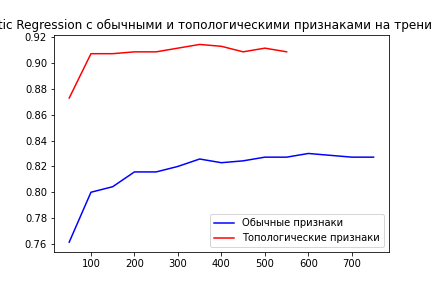
\includegraphics[width=\linewidth]{log_diff_features_train.png}
		\caption{Логистическая регрессия на тренировочной выборке}
		\label{fig:1}
	\end{subfigure}\hfil % <-- added
	\begin{subfigure}{0.25\textwidth}
		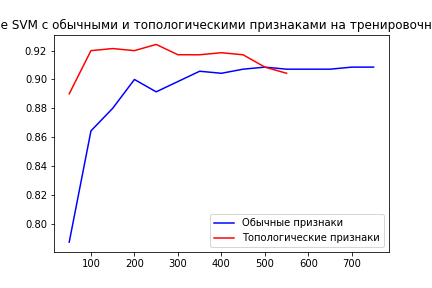
\includegraphics[width=\linewidth]{svm_diff_features_train.png}
		\caption{Метод опорных векторов на тренировочной выборке}
		\label{fig:2}
	\end{subfigure}\hfil % <-- added
	\begin{subfigure}{0.25\textwidth}
		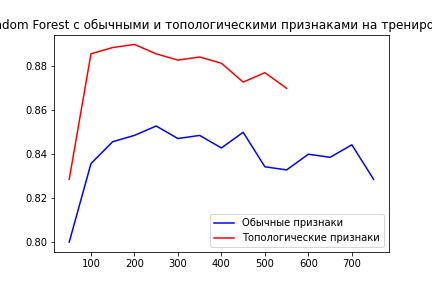
\includegraphics[width=\linewidth]{rf_diff_features_train.png}
		\caption{Случайный лес на тренировочной выборке}
		\label{fig:3}
	\end{subfigure}
	
	\medskip
	\begin{subfigure}{0.25\textwidth}
		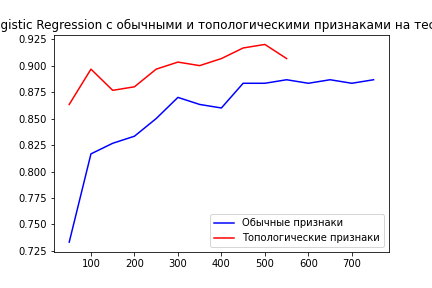
\includegraphics[width=\linewidth]{log_diff_features_test.png}
		\caption{Логистическая регрессия на тестовой выборке}
		\label{fig:4}
	\end{subfigure}\hfil % <-- added
	\begin{subfigure}{0.25\textwidth}
		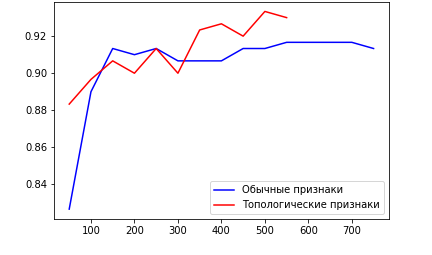
\includegraphics[width=\linewidth]{svm_diff_features_test.png}
		\caption{Метод опорных векторов на тестовой выборке}
		\label{fig:5}
	\end{subfigure}\hfil % <-- added
	\begin{subfigure}{0.25\textwidth}
		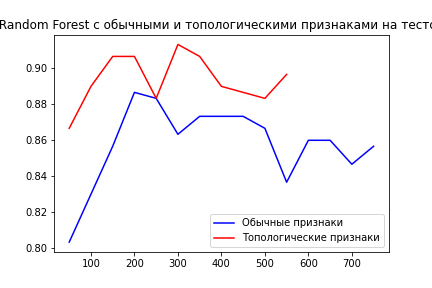
\includegraphics[width=\linewidth]{rf_diff_features_test.png}
		\caption{Случайный лес на тестовой выборке}
		\label{fig:6}
	\end{subfigure}
	\caption{Сравнение различных моделей, которые используют различные признаки}
	\label{accuracies_diff_features}
\end{figure}

Видно, что модели с топологическими признаками при малом количестве признаков достигает лучшей точности. Отсюда можно сделать вывод, что топологические признаки содержат в себе наиболее важную, релевантную информацию о структуре данных в меньшем числе признаков. Поэтому такой подход можно рассматривать как подход для уменьшения размерности данных. 

\begin{figure}[!htbp]
	\begin{center}
		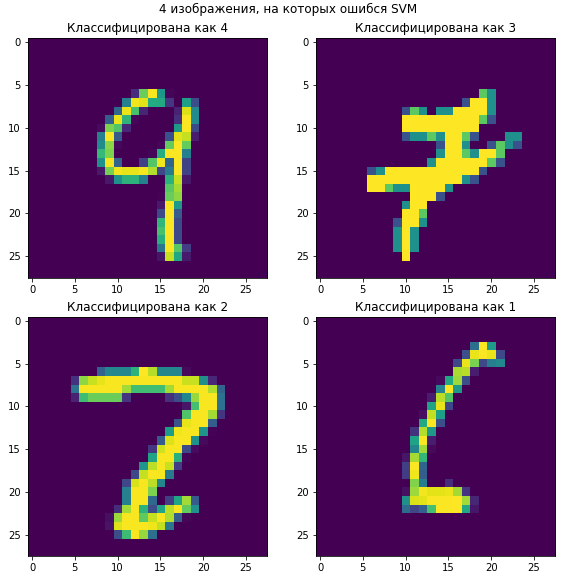
\includegraphics[width=0.75\textwidth]{missclassified.png}\\
		\caption{Первые несколько изображений, на которых ошибся классификатор}
		\label{missclassified}
	\end{center}
\end{figure}


Видно, что метод опорных векторов с подобранными параметрами на 400 лучших признаках, отобранных с помощью случайного леса, показывает чуть ли не самый высокий результат. Интересно посмотреть, на каких изображений эта модель ошиблась. На рис. \ref{missclassified} представлены как раз такие 4 изображения. Видно, что цифры, на которых ошибся классификатор, действительно похожи на те, которые классификатор предписал данным изображениях.
